\documentclass[12pt]{article}
\usepackage{times}
\usepackage[english]{babel}
\usepackage[utf8x]{inputenc}
\usepackage[colorinlistoftodos]{todonotes}
\usepackage[margin=1in]{geometry}
\usepackage{graphicx}
\usepackage{epstopdf}
\usepackage{cite}
\usepackage{listings}
\usepackage{dtklogos}
\usepackage{wrapfig}
\usepackage{subfigure}
\usepackage{amsmath}
\usepackage{amsthm}
\usepackage{amssymb}
\usepackage{amscd}
\usepackage{caption}
\usepackage{etoolbox}
\usepackage{fancyhdr}
\usepackage{stackengine}
\usepackage[export]{adjustbox}
\usepackage{rotating}
\patchcmd{\thebibliography}{\section*{\refname}}{}{}{}
\usepackage[document]{ragged2e}    %This causes text to left align
\usepackage[colorlinks=true, linkcolor=black,citecolor=black,urlcolor=blue]{hyperref}
\bibliographystyle{IEEEtran}
\extrafloats{100}
\DeclareGraphicsRule{.tif}{png}{.png}{`convert #1 `dirname #1`/`basename #1 .tif`.png}

\title{MCHE 357: Lab 9}

\begin{document}
\lefthyphenmin3
\righthyphenmin4
% \pretolerance=2000
% \tolerance=500 
% \emergencystretch=10pt
%\raggedright     %Stops LaTeX from automatically hyphenating the right margin to fit better
%Combine this with \usepackage[document]{ragged2e} to get a text align left similar to natural MS Word


%-------------------------------------------------------------
%Start of Paper
%-------------------------------------------------------------

%%%%%%%%%%%%%%%%%%%%%%%%%%%%%%%%%%%%%%%%%%%%%%%%%%%%%%
%%%%%%%%%%%%%%%%%%%%%%% TITLE PAGE %%%%%%%%%%%%%%%%%%%%%%%%
%%%%%%%%%%%%%%%%%%%%%%%%%%%%%%%%%%%%%%%%%%%%%%%%%%%%%%

\begin{titlepage}

\newcommand{\HRule}{\rule{\linewidth}{0.5mm}} % Defines a new command for the horizontal lines, change thickness here

\center % Center everything on the page
 
%----------------------------------------------------------------------------------------
%	Heading Section
%----------------------------------------------------------------------------------------

\textsc{\LARGE University of Louisiana at Lafayette}\\[1.5cm] % Name of your university/college
\textsc{\Large Measurements and Instrumentation}\\[0.5cm] % Major heading such as course name
\textsc{\large MCHE 357}\\[0.5cm] % Minor heading such as course title

%----------------------------------------------------------------------------------------
%	Title Section
%----------------------------------------------------------------------------------------

\HRule \\[0.4cm]
{ \huge \bfseries Lab 9}\\[0.4cm] % Title of your document
\HRule \\[1.5cm]
 
%----------------------------------------------------------------------------------------
%	Author Section
%----------------------------------------------------------------------------------------

\begin{minipage}{0.4\textwidth}
\begin{flushleft} \large
\emph{Author:}\\
\textsc{Matthew J. Begneaud} \\% Your name
\end{flushleft}
\end{minipage}
~
\begin{minipage}{0.4\textwidth}
\begin{flushright} \large
\emph{Professor:} \\
\textsc{Dr. Mostafa A. Elsayed} % Supervisor's Name
\end{flushright}
\end{minipage}\\[1.5cm]

% If you don't want a supervisor, uncomment the two lines below and remove the section above
%\Large \emph{Author:}\\
%John \textsc{Smith}\\[3cm] % Your name

%----------------------------------------------------------------------------------------
%	Date Section
%----------------------------------------------------------------------------------------

{\textsc{\large \today}}\\[0.5cm] % Date, change the \today to a set date if you want to be precise


%----------------------------------------------------------------------------------------
%	Group Section
%----------------------------------------------------------------------------------------
\textsc{\large Group:}\\[0.1cm]
\textsc{Ronald Kisor}\\
\textsc{Chandler Lagarde}\\
\textsc{Somto Umeokafor}
\\[0.5cm]

%----------------------------------------------------------------------------------------
%	Logo Section
%----------------------------------------------------------------------------------------


\includegraphics[width=5in]{UL_logo.jpg}\\[1cm] % Include a department/university logo - this will require the graphicx package
 
%----------------------------------------------------------------------------------------

\vfill % Fill the rest of the page with whitespace

\end{titlepage}

%%%%%%%%%%%%%%%%%%%%%%%%%%%%%%%%%%%%%%%%%%%%%%%%%%%%%%
%%%%%%%%%%%%%%%%%%%%%%% TABLE OF CONTENTS %%%%%%%%%%%%%%%%%%%
%%%%%%%%%%%%%%%%%%%%%%%%%%%%%%%%%%%%%%%%%%%%%%%%%%%%%%

\tableofcontents

\listoffigures

\bigskip


\section*{\fontsize{12}{12}\selectfont \large List of Symbols}
\addcontentsline{toc}{section}{List of Symbols} % Add for each section
None




\newpage

%%%%%%%%%%%%%%%%%%%%%%%%%%%%%%%%%%%%%%%%%%%%%%%%%%%%%%
%%%%%%%%%%%%%%%%%%%%%%% REPORT %%%%%%%%%%%%%%%%%%%%%%%%%%
%%%%%%%%%%%%%%%%%%%%%%%%%%%%%%%%%%%%%%%%%%%%%%%%%%%%%%


\section*{\fontsize{12}{12}\selectfont \large Introduction}
\addcontentsline{toc}{section}{Introduction} % Add for each section

This lab consisted of using Labview to create a program which reads data from a thermo-coupler to measure the temperature of an environment. The program was used to measure the ambient temperature of a room, the temperature between two fingers, and the temperature of a cold cup of water. 

\section*{\fontsize{12}{12}\selectfont \large Theory}
\addcontentsline{toc}{section}{Theory} % Add for each section

Labview can be used in conjunction with physical instruments in order to control a system or take data in from a system. Reading data from an instrument can be done by referring to the documentation of the instrument in order to map voltage readings to the desired measurement, while also considering the sensitivity of the instrument. 
\bigskip

A thermo-couple is a device used to measure temperature by use of material which changes resistance as its temperature changes. This changing resistance results in different voltages being outputted by the device which can then be mapped to temperatures. The mean voltage outputted at different temperatures is tabulated and can be read in the instrument's documentation. The user can simply interpolate to get temperatures that correspond to voltages that lie between the tabulated values.
\bigskip

\section*{\fontsize{12}{12}\selectfont \large Procedure \& Analysis}
\addcontentsline{toc}{section}{Procedure \& Analysis} % Add for each section

The program used in this lab would read the voltage outputted by the thermo-couple, shown in Figure 1, and map it to a temperature value by linearly interpolating the voltage with the data tabulated in the instrument's documentation. The temperatures recorded with the thermo-couple were compared to a reference thermometer, shown in Figure 2. The system diagram and control panel for the Labview program can be seen in Figure 3 and Figure 4, respectively. The data mentioned throughout this section can be seen tabulated in Figure 5. 
\bigskip

The temperature of the room was first measured and recorded with a physical reference thermometer. The thermo-couple was then used to measure the ambient temperature against a zero reference to determine the instrument's error. The error was then accounted for by the Labview program and the ambient temperature was measured again, this time resulting in the correct room temperature. 
\bigskip
 
 The reference thermometer was then used to measure and record the temperature between one lab member's finger tips. The same temperature was then measured with the thermo-couple. As can be seen in Figure 3, the temperatures closely match. 
\bigskip
 
The reference thermometer was then placed in a cup of cold water and the temperature was recorded. The temperature was then measured again using the thermo-couple. Again, the temperatures closely matched, as can be seen in Figure 3.
\bigskip

\newpage

\begin{figure}[h!] %  figure placement: here, top, bottom, or page
   \centering
   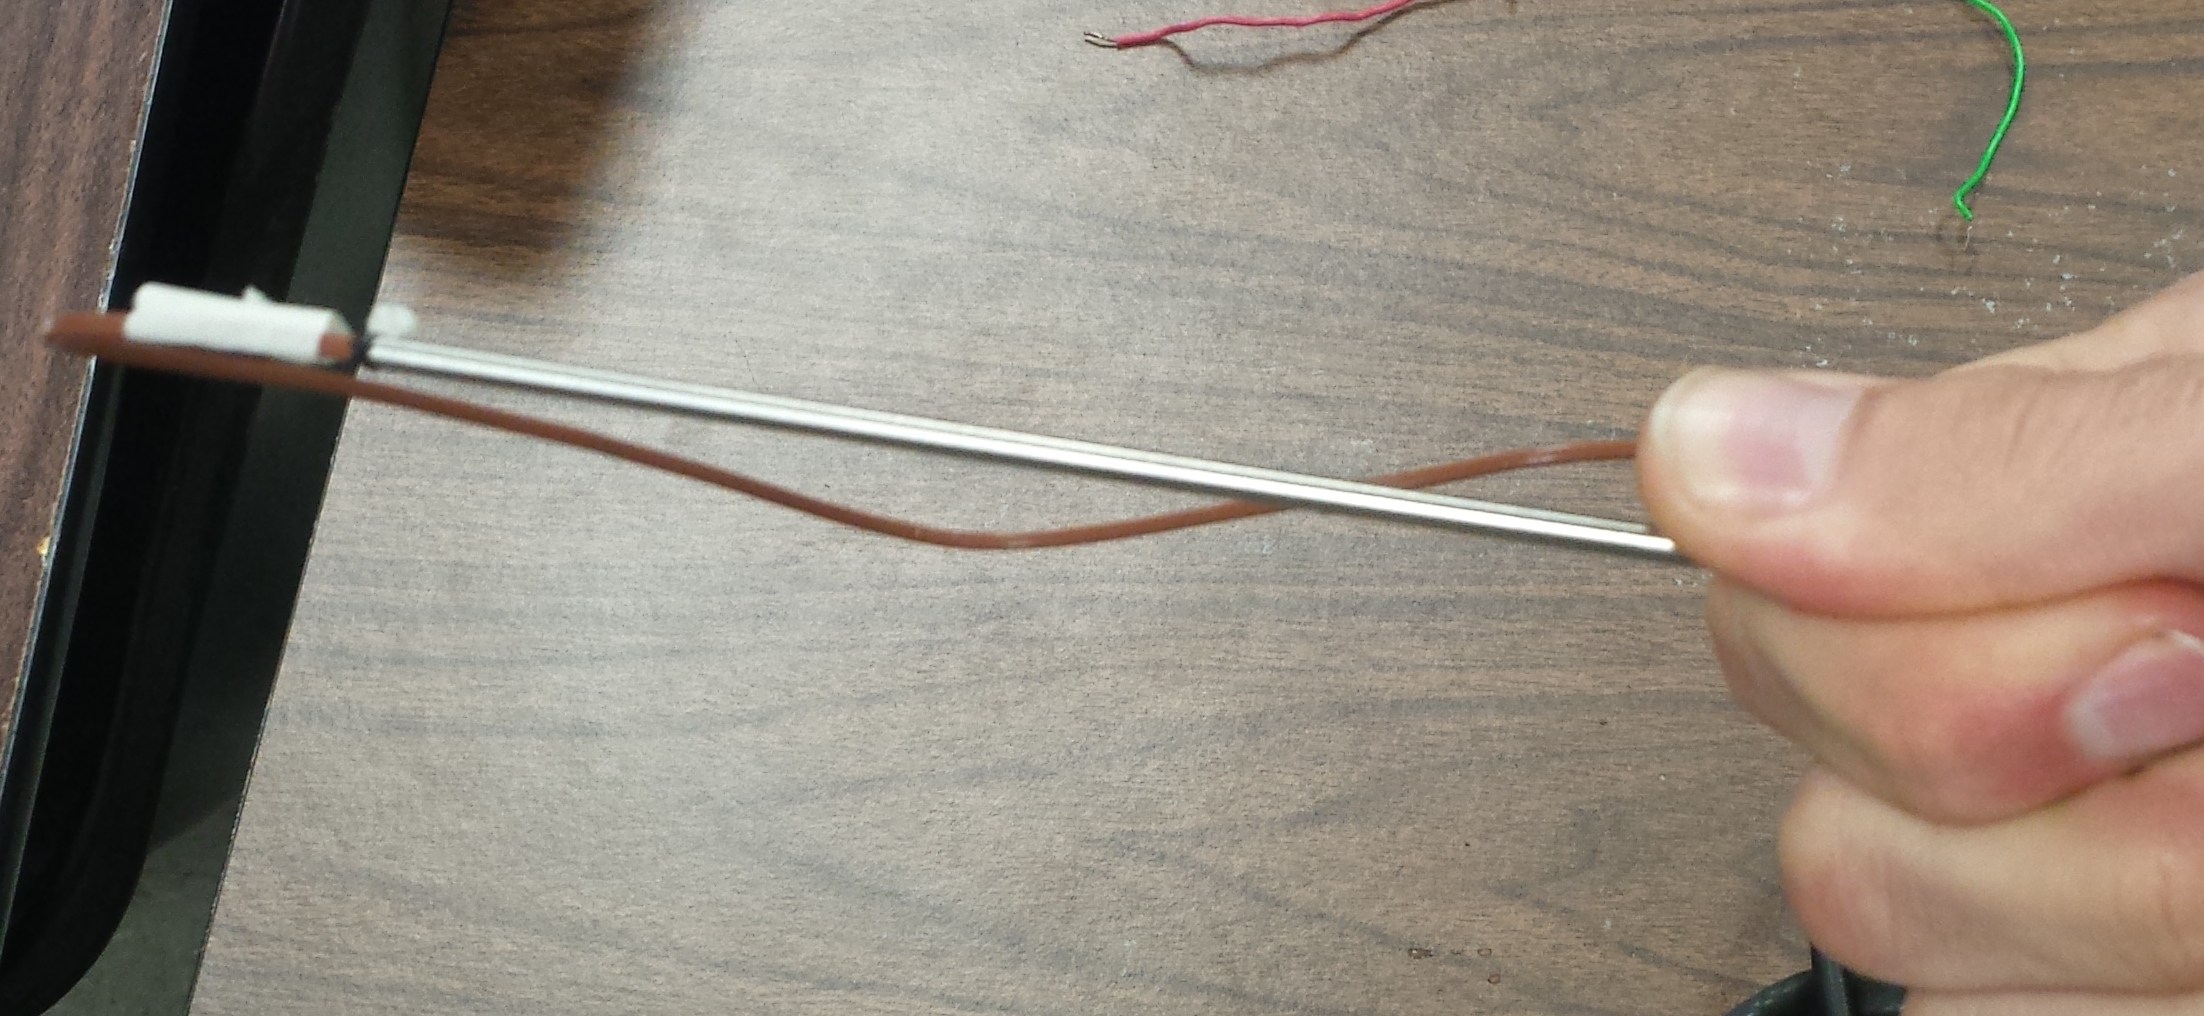
\includegraphics[width=\linewidth]{thermocouple.jpg} 
   \caption{Thermo-couple}
   \label{fig:example}
\end{figure}

\bigskip

\begin{figure}[h!] %  figure placement: here, top, bottom, or page
   \centering
   \includegraphics[width=\linewidth]{reference_thermometer.jpg} 
   \caption{Reference Thermometer}
   \label{fig:example}
\end{figure}

\newpage

\begin{figure}[h!] %  figure placement: here, top, bottom, or page
   \centering
   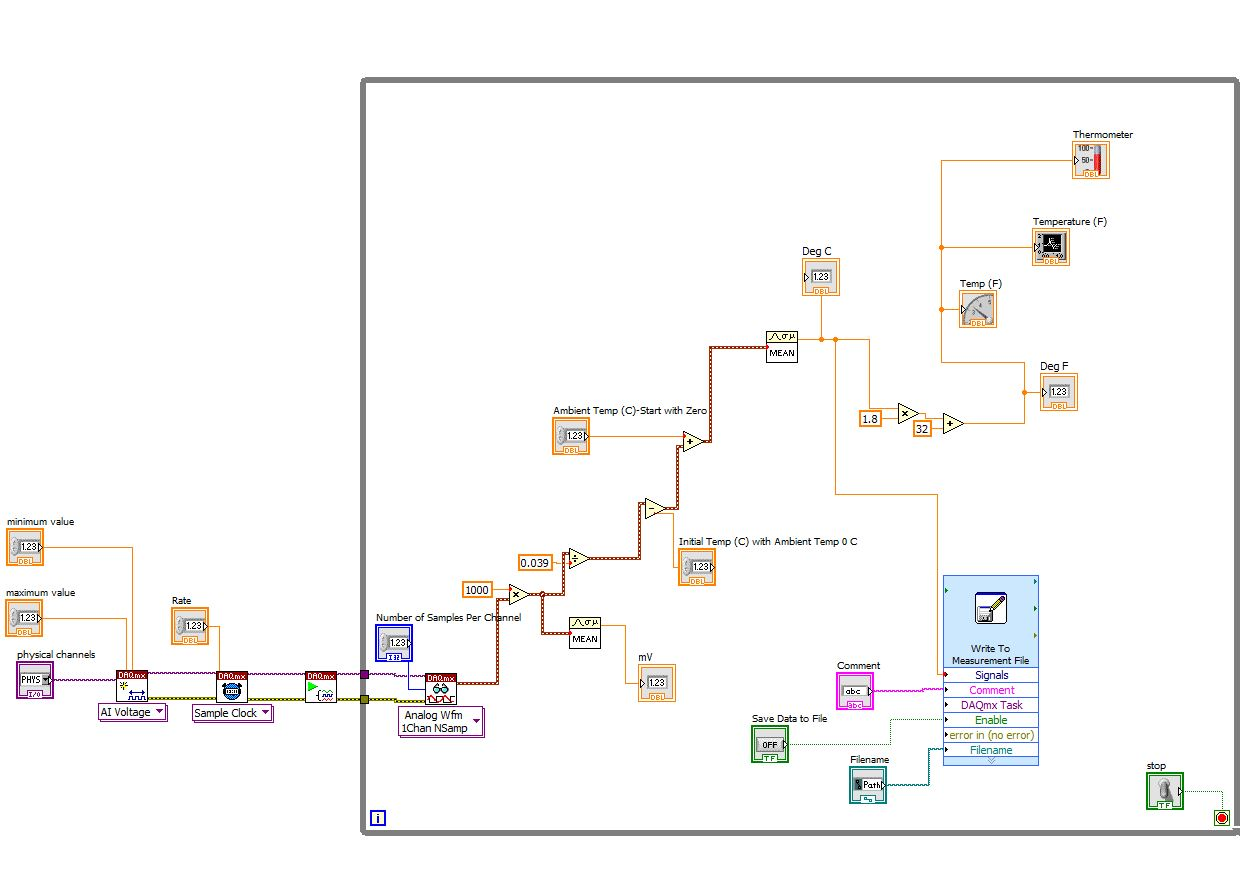
\includegraphics[width=\linewidth, height = 3.75in]{labview_system.jpg} 
   \caption{Labview System Diagram}
   \label{fig:example}
\end{figure}

%\bigskip

\begin{figure}[h!] %  figure placement: here, top, bottom, or page
   \centering
   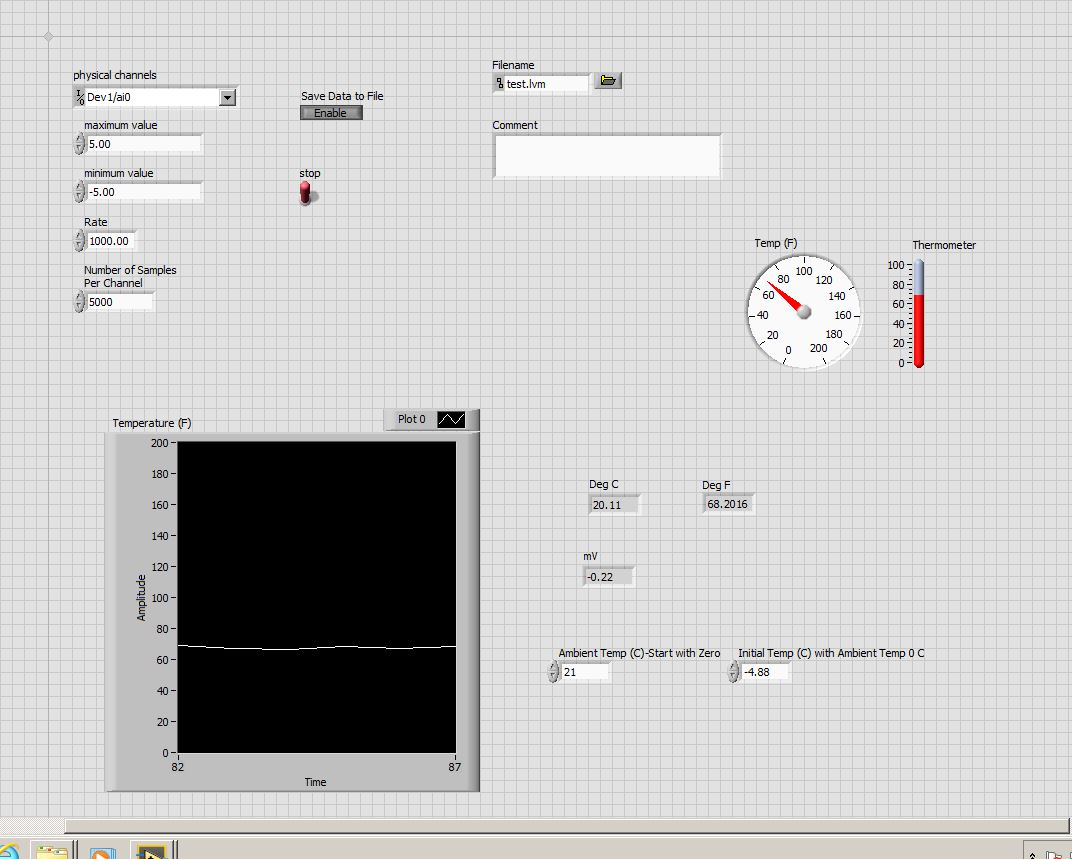
\includegraphics[width=\linewidth, height = 3.75in]{labview_control_panel.jpg} 
   \caption{Labview Control Panel}
   \label{fig:example}
\end{figure}

\newpage

\begin{figure}[h!] %  figure placement: here, top, bottom, or page
   \centering
   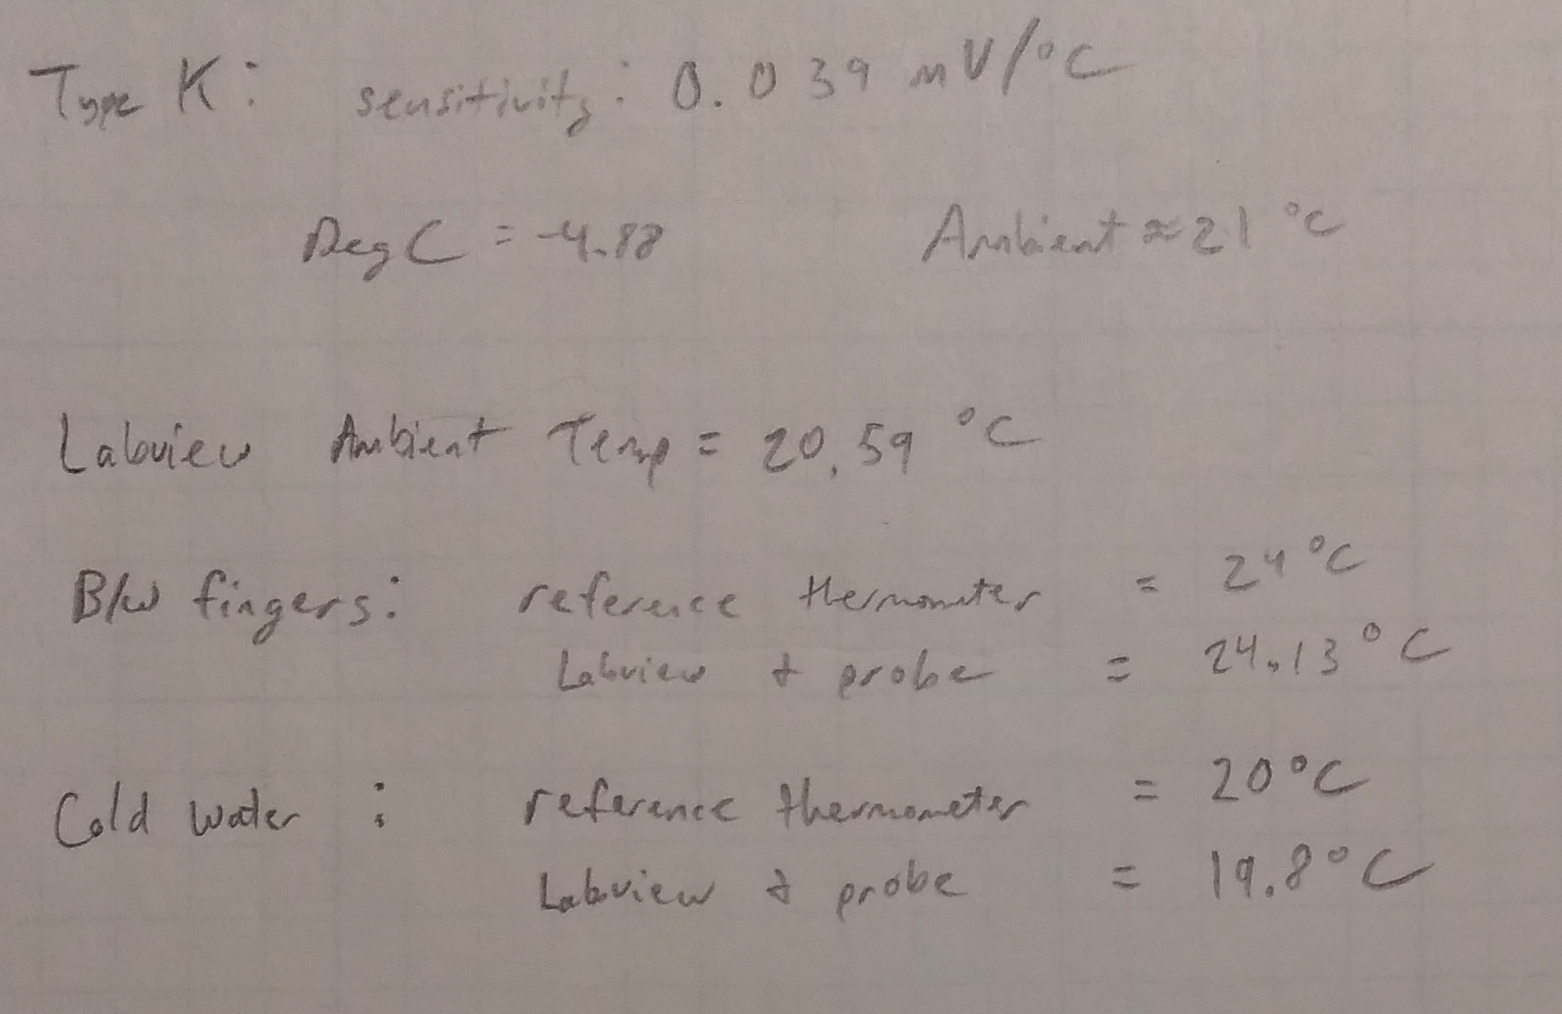
\includegraphics[width=\linewidth]{lab_notes.jpg} 
   \caption{Recorded Data \& Results}
   \label{fig:example}
\end{figure}

 
Overall, the thermo-coupler performed pretty well. However, for more accurate measurements, it would be wise to increase the sensitivity of the device because there was noticeable fluctuation every iteration of the Labview program reading the outputted voltage. The thermo-coupler also has a much higher range than necessary for the measurements made in this lab. A device with a smaller range would be more effective, as more resolution could be achieved across the spectrum of voltage readings.
\bigskip


\section*{\fontsize{12}{12}\selectfont \large Conclusion}
\addcontentsline{toc}{section}{Conclusion} % Add for each section
The exercises conducted in this lab demonstrated using a Labview program to acquire data. It was shown that reading data from sensors is typically done by mapping the voltage reading from the sensor to a measurement value by using documentation on the specific sensor being used. This is how most measurement systems work, and it is important that students are exposed to using these sensors as they will likely use them in their careers in the industry. Exhibiting this method by use of a temperature measuring device is good because these types of devices are commonly used, even outside of the engineering world. 


%\section*{\fontsize{12}{12}\selectfont \large References}

%\begin{thebibliography}{2}
%
%% Example
%%\bibitem{Wagner}
%%Ng, K., Wagner, S.W., Camelio, J., Emblom, W.J. (2010). ?Experimental Analysis of Micro Tube
%%Hydroforming Process.? Transactions of NAMRC of SME, 38, 577-584.
%
%\end{thebibliography}



%\section*{\fontsize{12}{12}\selectfont APPENDIX}

%\begin{table}[h!]
%  \caption{}
%  \includegraphics[width=\linewidth]{table1.png}
%\end{table}




\end{document}







----------------------------Templates-------------------------------

-------------------------Figure-----------------------

\begin{figure}[h!]  
  \centering
    \includegraphics[width=\linewidth]{**file**}
    \caption{Docking Station}
\end{figure}

---------------------------Table-----------------------
\begin{table}[ht]
\caption{Nonlinear Model Results} % title of Table
\centering % used for centering table
\begin{tabular}{c c c c} % centered columns (4 columns)
\hline\hline %inserts double horizontal lines
Case & Method\#1 & Method\#2 & Method\#3 \\ [0.5ex] % inserts table
%heading
\hline % inserts single horizontal line
1 & 50 & 837 & 970 \\ % inserting body of the table
2 & 47 & 877 & 230 \\
3 & 31 & 25 & 415 \\
4 & 35 & 144 & 2356 \\
5 & 45 & 300 & 556 \\ [1ex] % [1ex] adds vertical space
\hline %inserts single line
\end{tabular}
\label{table:nonlin} % is used to refer this table in the text
\end{table}



probably best to insert as an image from excel

\bigskip\\
\begin{table}[h!]
  \caption{}
  \includegraphics[width=\linewidth]{**file**}
\end{table}
\bigskip\\





-----------------------------Equations------------------------
-----------------------------Regular
\begin{equation}
a = b + c
\end{equation}

--------------------------------- Multiline
\begin{multline}
a = b + c + d + e + f
+ g + h + i + j \\
+ k + l + m + n + o
\end{multline}

-------------------------------Citations-------------------------
\bibitem{Author last name}
  Last, First., year of publication,
  article name, book(etc) name, from \\
  link goes here

----------------------------------other-----------------------------

equations:
http://moser-isi.ethz.ch/docs/typeset_equations.pdf

citations:
http://library.missouri.edu/engineering/about/guides/asme
https://www.asme.org/shop/proceedings/conference-publications/references